\chapter{基于LOF的流式数据异常检测方法研究}
\label{chap:intro}
上节内容介绍了异常数据检测的几种方法,并介绍了如何对流式数据进行处理。可以看出,在这些异常数据检测方法中,基于统计的检测方法需要假定数据集服从特定的概率分布,然而在现实应用中,数据的分布情况一般较为复杂,而且通常随着时间会有变化,不是始终如一的,很难得到数据的分布。基于聚类的方法只能给出数据点是否是异常点的判断,不能量化数据点的异常程度,而且异常检测是聚类的“副产品”,很难对异常检测做到优化。而基于密度的LOF算法,可以很好地量化数据点的异常程度,并且能较好地识别异常点。

\section{LOF方法及增量的LOF方法}
Breunig和Ng等人发现,之前已存在关于异常检测的研究中,都把异常点当做是一个二分属性,对象只能分为是异常的或不是异常的,他们认为,在一些场景下,给出一个对象是异常点的度更有意义,这个度被称为局部异常因子,简称$LOF$,并且提出一种算法,称为LOF算法\upcite{Breunig2000LOF}。为了证明LOF算法的优越性,他们提出了如下一个问题。如图\ref{fig:fig32}所示,是一个二维数据集,其中包括两个类$C_1$和$C_2$,还有两个游离在外的数据点$o_1$和$o_2$。从中可以看出$C_1$类中数据比较稀疏,$C_2$类中数据比较密集。异常数据检测的目的,应该在整个数据集中找出异常数据点$o_1$和$o_2$。可以很明显地看出,数据集的分布不规律,不能使用基于统计的方法,而使用基于聚类的方法,如果把$C_1$中的点聚为一类,则也会把$o_2$点聚类到$C_2$中,只能识别$o_1$点为异常点。如果使用基于距离的方法,可以看出,$o_2$距离类$C_2$中的数据点的距离要小于$C_1$类中的某些点距离其邻近点的距离,如果距离阈值设置较大,则数据点$o_2$不会被检测为异常数据点,如果阈值设置较小,数据点$o_2$会被认为是异常数据点,但类$C_1$中的许多数据点也会被误认为是异常数据点。所以,基于距离的方法也不能准确地识别出异常点。基于密度的方法也存在这样的问题,数据点$o_2$周围点的数量不少于位于类$C_1$中的数据点,数据点$o_2$的密度不小于位于类$C_1$中的数据点的密度。而LOF方法可以解决这类问题。

\begin{figure}
	\centering
	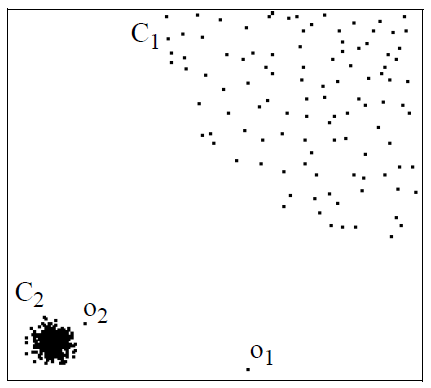
\includegraphics[width=0.35\textwidth]{figures/figure3x2}
	\caption{一个二维数据集}\label{fig:fig32}
\end{figure}

LOF方法中$LOF$的定义为局部异常因子,它依赖于对象周围邻居的分布情况,是邻居结点的密度与自身密度的比值,$LOF$值越高,表明邻近对象都处于一个密集的状态,而本身密度较低,说明这个对象越可能是异常点,如数据点$o_2$。$LOF$越接近1的话,表明该对象所处区域的密集程度与邻近对象越一致,说明这个对象越不可能是异常点,如位于类$C_1$中的数据点。关于LOF算法,解释如下。

定义1 $\ d(p, q)$:对象$p$ 和对象$q$之间的欧式距离。

定义2 $\ k-distance(p)$:对象$p$的$k$距离,是对象$p$和对象$o$之间的距离$d(p, o)$,且满足

(1) 在数据集中至少有$k$个对象$o^{'}$,满足$d(p,o^{'})\leq d(p,o)$;

(2) 在数据集中最多有$k-1$个对象$o^{'}$,满足$d(p,o^{'}) < d(p,o)$。

其中,$k$是任意的正整数。

定义3 $\ N_{k-distance}(p)$:对象$p$的$k$近邻,其中的每一个对象$q$都满足$d(p,q)\leq k-distance(p)$。一个对象$p$的$k$近邻,可以被记住$kNN(p)$。

定义4 $\ reach-dist_k(p,o)$:对象$p$到$o$的可达距离。如果$p$是$o$的$k$近邻内的点,则$p$到$o$的可达距离为对象$o$的$k$距离,否则,$p$到$o$的距离是$d(p, o)$,即,
 \begin{equation}reach-dist_k(p, o) = max\left \{ k-distance(o), d(p, o) \right \}\end{equation}

如图\ref{fig:fig31}所示, $\ k=3$,则对象$p$的$k$距离就是$d(p, q_3)$,对象$p$的$k$近邻$N_{k-distance}(p) = \left \{ q_{1}, q_{2}, q_{3} \right \}$,
$reach-dist_k(q_2, p) = k-distance(p) = d(q_3, p)$,而$reach-dist_k(q_4, p) = d(q_4, p)$。
\begin{figure}
	\centering
	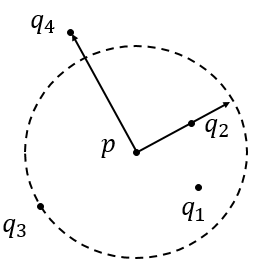
\includegraphics[width=0.25\textwidth]{figures/figure3x1}
	\caption{$k=3$时,点$q$的$k$邻域}\label{fig:fig31}
\end{figure}

定义5$\ $局部可达密度$(lrd)$:对象$p$的局部可达密度定义为
\begin{equation}
lrd_{k}\left ( p \right ) = 1 / \left ( \frac{\sum_{o\in N_{k}\left ( p \right )}reach-dist_{k}\left ( p,o \right )}{\left | N_{k}\left ( p \right ) \right |} \right )
\end{equation}

定义6$\ $局部异常因子$(LOF)$:对象$p$的局部异常因子定义为
\begin{equation}\label{equ:lof}
LOF_{k}\left ( p \right ) = \frac{\sum_{o\in N_{k}\left ( p \right )}\frac{lrd_{k}\left ( o \right )}{lrd_{k}\left ( p \right )}}{\left | N_k\left ( p \right ) \right |}
\end{equation}

对象的局部异常因子$(LOF)$代表了一个对象的异常程度,由式子\ref{equ:lof}可知,一个对象的异常因子是该对象的邻居对象的平均密度与该对象的密度的比值,如果该值接近于1,则表明该对象很可能是个正常的数据点,而该值越大,则越表明该对象可能是异常的。此时,对异常值的判断有了个程度的表示,于是可以通过控制阈值的大小,来检测不同粒度的异常数据。

当检测流式数据时,为了避免计算效率低下或者算法导致不正确的结果,LOF算法需适应流式数据的特点。一般来说,LOF算法用于流式数据可以有以下几种方式。

第一种方法,每次数据点到来后,对数据集进行一次静态的LOF算法检测,这种方法可以精确地检测出此数据是否为异常数据,但是计算量庞大。每次新数据点到来后,都要对整个数据集进行一次计算,计算每个点的$LOF$值。LOF算法的时间复杂度是$O(n\log n)$\upcite{Breunig2000LOF},如果当前的数据集的数据点的个数为$N$,则进行了$N$次检测,则总共的时间复杂度为\upcite{Pokrajac2007Incremental}
\begin{equation}O\left ( \sum_{n=1}^{N}n\log n \right ) = O\left ( N^{2}\cdot \log N \right )\end{equation}
由此可以看出,这种方法虽然简单,当一个异常数据到来之后,可以立刻检测出来,但是,计算复杂度太大。

第二种方法对第一种方法进行了改进,不再是每当一个数据点到来后进行LOF算法检测,而是当一批数据点到来之后,再进行检测。数据流是动态的,源源不断的,且无法全部缓存的,而LOF算法是静态的算法,适用于一个数据集的,那么可以将数据流依次缓存,定期地使用LOF算法,每当一定数量的数据点到达后,对整体数据点使用LOF算法检测\upcite{Domingos2003A}。这种方法比较简单,相当于把数据流分为了多个数据集,把动态的数据流变成了静态的数据集。但是计算复杂度依旧比较高,而且,这种方式对于检测具有延迟性,不能立刻检测出异常数据。

第三种方法引入滑动窗口的思想,每次只对窗口内的数据进行异常数据检测。这种方法相当于设置一个缓存区,将数据流缓存下来,缓存到一定的大小后,对其进行LOF算法检测。之后再进行缓存,周期性地进行LOF算法检测。这种方法计算复杂度不高,但是同样具有检测延迟的问题,而且,这种方法只检测缓存区中的数据,缓冲区的大小相当于对数据流的分割的块的大小。没有考虑历史数据的影响,很可能将正常数据点检测为异常的数据。

为了改进上面这些方法的不足,Pokrajac提出了一种针对流式数据的增量式的异常因子检测算法(增量LOF算法)\upcite{Pokrajac2007Incremental},这种方法与第一种方法相似,每次新插入一个数据点后都需要计算局部异常因子,这样对数据的检测不具有延迟性,可以实时检测数据的异常度,但是不同的是,该方法通过数学推论,引入了$kRNN$的定义,每次只更新计算新插入的数据点及其影响到的数据点,减少了计算复杂度。假设有对象$p$,则$kRNN(p)$定义为,所有的$k$邻域中包含$p$的对象点的集合,即如果对象$p$是对象$o$的$k$近邻内的一个点,则对象$kRNN(p)$包含对象$o$。当插入一个新的数据点时,该方法的伪代码\upcite{Pokrajac2007Incremental}如算法\ref{alg:lof}所示。

\begin{algorithm}%
	\KwIn{stream data $S\  {p_1, ..., p_n}$}
	
	\KwOut{the $LOF$ of data}
	%\SetVline
	\While{insert($p_c$)}{
		Compute $kNN(p_c)$\;
		\For{$\forall p_j \in kNN(p_c)$}{
			compute $reach-dist_k(p_c, p_j)$\;
		}
		//Update neighbors of $p_c$ \\
		$S_{update\_k\_distance} = kRNN(p_c)$\;
		\For{$\forall p_j \in S_{update\_k\_distance}$}{
			update $k-distance(p_j)$\;
		}
		$S_{update\_lrd} = S_{update\_k\_distance}$\;
		\For{$\forall p_j \in S_{update\_k\_distance}$, $\forall p_i \in kNN(p_j)\setminus \left \{ p_c \right \}$}{
			$reach-dist_k(p_i, p_j) = k-distance(p_j)$\;
			\If{$p_j \in kNN(p_i)$}{
				$S_{update\_lrd} = S_{update\_lrd} \cup  \left \{ p_i \right \}$\;
			} 
		}
		$S_{update\_LOF} = S_{update\_lrd}$\;
		\For{$\forall p_m \in S_{update\_lrd}$}{
			update $lrd(p_m)$\;
			$S_{update\_LOF} = S_{update\_LOF} \cup  kRNN\left \{ p_m \right \}$\;
		}
		\For{$\forall p_l \in S_{update\_LOF}$}{
			update $LOF(p_l)$\;
		}
		compute $lrd(p_c)$\;
		compute $LOF(p_c)$\;
	}
    \caption{增量LOF算法}
    \label{alg:lof}
\end{algorithm}

该增量LOF算法的时间复杂度为$O\left (N\cdot \log N \right )$,时间复杂度较低,而且在每次来一个数据点后都可以计算其局部异常因子,可以找到异常值,不具有延迟性,而且其准确度跟静态LOF算法一样,既可以考虑到历史数据的影响,又不会因为数据分段而造成将正常数据误认为是异常数据的情况。但是在流式环境下,该方法依旧存在问题,那就是计算时间与存储的问题。虽然这种方法在每来一个数据点后,都是只更新该数据点影响到的数据点,但是,全体数据量随着时间越来越多,一段时间后,达到海量的数据量,此时,如果不丢弃数据点,每次数据点$o$到来后,都需要计算数据点$o$的$k$邻域,$kNN$和$kRNN$序列,以及需要计算$k$邻域包含$o$的所有数据点,并且计算更新这些数据点的$kNN$和$kRNN$,所以检测的时间也会越来越大,会造成计算缓慢。如果丢弃掉历史上的部分数据点,只选取近一段时期内的数据点,又会造成不精确的结果,甚至造成误报。而且会造成存储容量不够的问题。这些数据点都是存储在内存中的,一段时间后,数据越来越多,内存存储容量不够,会引起数据丢失和无法进行检测的后果。为了解决这个问题,我们提出了一种既可以在线检测,实时检测异常数据,又可以解决数据量很大内存容量不够计算时间长等问题的新的方法。

\section{改进的增量LOF快速检测算法}
由上文可知,流式数据的特性是数据量庞大,当时间越来越长后,接收到的数据量越来越多,数据存储在内存中进行异常数据检测,此时,会造成两个问题:(1)存储空间问题,流式数据全部存储在内存中基本是不可能的。(2)计算问题,当数据存储在内存中后,内存资源变少,会造成计算资源减少的问题,而且当数据量越来越多时,算法的运行时间也越来越长。为了解决这两个问题,本文提出一种改进的增量LOF快速检测算法,不但能够快速实时地计算新来数据点的局部异常因子,检测异常数据,也可以解决流式数据的数据存储问题。

该算法考虑到流式数据数据量巨大的特性和异常数据“少而不同”的特点,认为,选取一个较小的数据子空间,当该子空间与数据空间相比足够小时,子空间中的数据点可以认为是分布在同一位置的。所以,本算法主要是将数据空间划分为网格,并将映射到网格中的数据点,看做是落在网格中的同一位置,即将网格某位置的数据点,作为本网格的代表点,来代表落在本网格的所有数据点。并且调整LOF算法,使其适应于网格模式下的数据点。

本节内容主要介绍算法的实现,包括网格的定义与划分,网格的特征向量的定义以及坐标的选择,数据点如何映射到网格中,数据点映射到网格中后选取哪一点作为代表点,代表点如何反映该网格的数据点的数量,以及在算法实现过程中,关于LOF算法的相关概念的重新定义等。本算法可以分为两个模块,一个模块在线接收数据,并且将数据映射到相对应的网格中。一个模块来进行计算,对到来的数据所影响的网格进行更新,计算新来的数据点的异常因子。以下来详解介绍该方法的实现。
%说明一下用网格中的一个带有权重的点来代替网格中的所有点
\subsection{网格定义及划分}
流式数据因为存储问题无法保存所有的原始数据,但是如果将流式数据所在数据空间划分为一个个的网格,将数据点映射到对应的网格中,更新网格的特征值,用网格来代替其中所有的数据,就可以解决这个问题。所以该方法将数据空间划分为网格,使用网格来保存数据的概要信息。假设流式数据$S$的维度为$D$,流式数据的属性值空间为
\begin{equation}
S = S_1\times S_2 \times ... \times S_D
\end{equation}
其中,$S_i$为第$i$维空间, $i = 1, 2, ..., D$。
将数据空间划分为网格,假设第$i$维的长度为$l_i$,划分的每一段的长度为$d_i$,可以将空间的第$i$维均匀地划分为等长的$n_i$段,即
\begin{equation}
S_i = S_{i,1} \cup S_{i,2} \cup ... \cup S_{i, n_i}
\end{equation}
其中,$l_i = d_i * n_i$。此时,整个数据空间$S$被划分为网格,第$i$维被划分为$n_i$段,则整个数据空间被划分为$\prod_{i=1}^{D}n_i$个网格。每个网格$G$由每一维度上的一段$S_{i, j_i}$共同构成,记作:
\begin{equation}
G = \left ( S_{1,j_1}, S_{2,j_2},...,S_{D,j_D} \right )
\end{equation}
其中,$j_i = 1, 2, ..., n_i$。

\subsection{网格的特征向量}
在本文中,一个网格的特征向量被定义为$(C, w, reachDis, knn, krnn, lrd, LOF)$,如表格\ref{tab:grid}所示,其中$C$是网格的坐标向量,$w$是网格的权重,代表该网格中数据点的数量,$reachDis$是网格的$k$邻域的可达距离,$knn$和$krnn$是两个序列,分别存储$k$邻域内所包含的网格的集合和所有的$k$邻域中包含该网格的网格的集合,$lrd$是该网格的局部可达密度,$LOF$是该网格的局部异常因子。

\begin{table}
	\centering
	\caption{网格的特征向量符号及其含义} \label{tab:grid}
	\begin{tabular*}{0.9\textwidth}{@{\extracolsep{\fill}}cccc}
		\toprule
		符号			&含义 \\
		\midrule
		$C$			&网格的坐标向量 \\
		$w$			&网格的权重 \\
		$reachDis$	&$k$邻域的可达距离 \\
		$knn$	&$k$邻域包含的网格的集合 \\
		$krnn$			&$k$近邻包含该网格的网格的集合 \\
		$lrd$			&网格的局部可达密度 \\
		$LOF$	&网格的局部异常因子 \\
		\bottomrule
	\end{tabular*}
\end{table}

%定义relatedGrid结构
\subsection{网格的坐标以及代表点}
网格的坐标向量用来确定一个网格的位置。当数据点映射到网格中时,需要确定映射到的网格。确定一个网格也就是确定网格的坐标向量。假设一个网格的坐标向量为
\begin{equation}
g = \left (j_1, j_2, ..., j_D \right )
\end{equation}
网格的坐标向量表示有以下两种方式,如图\ref{fig:fig34}所示,左边的坐标向量表示方式是将网格各个维度最小值的坐标值的向量作为网格本身的坐标值向量,也就是说,该网格表示的数据空间的各个维度的范围为$[j_1 * d_1, j_1 * d_1 + d_1), [j_2 * d_2, j_2 * d_2 + d_2), ... [j_D * d_D, j_D * d_D + d_D)$。右边的坐标向量表示方式是将网格的形心的坐标作为网格本身的坐标值,也就是说,该网格表示的数据空间的各个维度的范围为$[j_1 * d_1 - 0.5 \ast d_1, j_1 * d_1 + 0.5 \ast d_1),[j_2 * d_2 - 0.5 \ast d_2, j_2 * d_2 + 0.5 \ast d_2), ..., [j_D * d_D - 0.5 \ast d_D, j_D * d_D + 0.5 \ast d_D)$。

假设有一个二维空间的数据序列,数据空间划分网格的方式分别采用图\ref{fig:fig34}中所示的两种方式。

\begin{figure}[htb]
	\centering
	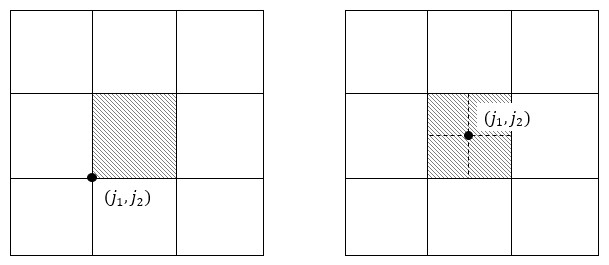
\includegraphics[width=0.35\textwidth]{figures/figure3x4}
	\caption{两种网格坐标表示}\label{fig:fig34}
\end{figure}

假设数据点$(x_1, x_2)$可以映射到网格$g={j_1, j_2}$,为方便计算,假设其误差为距离的平方和,即
\begin{equation}
f = \left ( (x-j_1*d_1)^2 + (y - j_2* d_2)^2 \right )
\end{equation}
则第一种方式中,网格的坐标向量是各维度表示范围的最小值的坐标值的向量,则其总误差如式子\ref{equ:equ310}所示:
\begin{equation}\label{equ:equ310}
\begin{split}
R_1 &= \int_{j_2d_2}^{j_2d_2 + d_2}\int_{j_1d_1}^{j_1d_1 + d_1}((x - (j_1d_1))^{2} + (y - (j_2d_2))^2){\mathrm{d} x}{\mathrm{d} y}\\
 &= \frac{1}{3}d_{1}d_{2}\left ( d_1^2 + d_2^2 \right )
\end{split}
\end{equation}
在第二种方式中,网格的坐标向量是网格形心的坐标向量,则其总误差如式子\ref{equ:equ311}所示,
\begin{equation}\label{equ:equ311}
\begin{split}
R_2 &=\int_{j_2d_2 -0.5d_2}^{j_2d_2+0.5d_2}\int_{j_1d_1-0.5d_1}^{j_1d_1+0.5d_1}((x-j_1d_1)^2+(y-j_2d_2)^2){\mathrm{d} x}{\mathrm{d} y} \\
 &= 4 * \int_{j_2d_2}^{j_2d_2+0.5d_2}\int_{j_1d_1}^{j_1d_1+0.5d_1}((x-j_1d_1)^2+(y-j_2d_2)^2){\mathrm{d} x}{\mathrm{d} y} \\
 &= \frac{1}{4}\ast \frac{1}{3}d_{1}d_{2}\left ( d_1^2 + d_2^2 \right )
\end{split}
\end{equation}
由式子\ref{equ:equ310}和式子\ref{equ:equ311}可知,第二种方式中,数据映射到网格中用网格坐标代替后,其误差更小。所以,本文选择第二种方式来表示网格。第二种方式实际上是用网格的形心点的坐标向量作为网格的坐标向量。

当数据点到来时,确定其映射到的网格过程如下,假设新的数据点$x = (x_1, x_2, ... x_D)$,则第$i$维的值$x_i$,将其做如下转换:
\begin{equation}
	j_i = \left \lfloor x_i / d_i + 0.5 \right \rfloor
\end{equation}
从而得出数据点$x$所属的网格$g = (j_1, j_2, ... , j_D)$

网格代表点的选取应该使得该点代表其他数据点时误差最小。如图\ref{fig:fig36}所示,是一个二维网格,第一维长度为$d_1$,第二维长度为$d_2$,且$d_1, d_2 >0$。

\begin{figure}[htb]
	\centering
	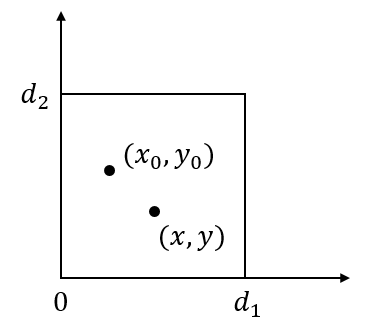
\includegraphics[width=0.35\textwidth]{figures/figure3x6}
	\caption{二维网格,代表点为$\left ( x_{0},y_{0} \right )$,任意一数据点$(x,y)$}\label{fig:fig36}
\end{figure}

假设网格代表点为$\left ( x_{0},y_{0} \right )$, 网格中任意一点为$(x,y)$,且满足$0\leq x,x_0\leq d_1, 0\leq y,y_0\leq d_2$。假设网格中数据点均匀分布,则其误差可定义为

\begin{equation}
\begin{split}
R &=\int_{0}^{d_2}\int_{0}^{d_1}\left ( \left ( x-x_0 \right )^2 + \left ( y-y_0 \right )^2 \right )\mathrm{d} x\mathrm{d} y \\
&=\frac{1}{3}d_2\left ( \left ( d_1-x_0 \right )^3+x_{0}^{3} \right )+\frac{1}{3}d_1\left ( \left ( d_2-y_0 \right )^3+y_{0}^{3} \right )
\end{split}
\end{equation}
因为$0\leq x_0\leq d_2$,$0\leq y_0\leq d_2$,则当$x_0=\frac{1}{2}d_1, y_0=\frac{1}{2}d_2$时,误差$R$最小。所以,代表点的坐标也就是该网格形心的坐标向量,这种情况可以扩展到多维空间。所以网格的坐标向量和代表点的坐标向量都是网格形心的坐标向量,因此,在网格的特征向量中,用$C$来代替网格的坐标向量和代表点的坐标向量,统称为网格的坐标向量。

为了区分不同网格中数据点的数量,引入权重的概念,也就是网格的特征向量中的$w$,代表了该网格中数据点的个数。从以上内容可知,将数据点映射到对应的网格中,然后用该网格的具有权重值的形心点代替所有的数据点来进行下一步的计算。

\subsection{算法实现}
流式数据的数据量巨大,而且一般为高维数据。将数据空间划分为网格时,海量数据映射到网格中。此时,当网格相比于数据空间足够小时,同一个网格中的数据点,在空间上和属性上具有相似性,可以将这些映射到同一个网格中的数据点看做是一样的数据点,所以这些数据点可以用一个带有权重的数据点来近似表示。这个数据点是网格的坐标,而权重是网格内已存的数据点的个数。此时,LOF算法中的数据点不再是单个的数据点,而是具有权重的数据点,所以,对其进行重新定义。

定义7$\ d^{'}\left ( p,q \right )$:网格$p$和网格$q$之间的距离,设网格$p$的坐标向量为$(p_1, p_2, ..., p_D)$,网格$q$的坐标向量为$(q_1, q_2, ..., q_D)$,则网格$p$和网格$q$之间的距离定义为
\begin{equation}
d^{'}(p,q) = (\sum_{i=1}^{D}(p_i - q_i)^{2})^{\frac{1}{2}}
\end{equation}

定义8$\ w_p$:网格$p$的权重,也可以称为网格$p$的密度,是网格$p$中数据点的个数。

定义9$\ k-distance^{'}(p)$:网格$p$的$k$距离,是网格$p$和网格$o$之间的距离$d(p, o)$,且满足

(1) $\sum  w_{o_i} < k $,其中$w_i$是网格$ w_{o_i}$的权重,且满足$d(p,o_i)\leq d(p,o)$。

(2) $\sum  w_{o_i} + w_o >= k$,其中$ w_{o_i}$是网格$o_i$的权重,满足$d(p,o_i)\leq d(p,o)$,$w_o$是网格$o$的权重。

此时有两种情况出现,如图\ref{fig:fig35}所示,一种是$\sum w_i + w_o = k$,则网格$o$正好全部包括在网格$p$的$k$邻域内,且是网格$p$的$k$邻域的边界,此时对象$p$的$knn$包括网格$o$。一种是$\sum w_i + w_o > k$,此时网格$o$正好横跨在网格$p$的$k$近邻线上。如果网格$o$中有$100$个数据点,而网格$p$有$98$个数据点,$k=100$,此时,如果网格$p$的$k$近邻包括$o$,则$k$近邻一共有$198$个数据点,极为不精确。为了计算的准确性,本文假设每个网格中的数据均匀分布,并为每一个网格$g$的$k$近邻网格的序列$knn$中加了一个属性$Score$,称为比值,表示$knn$中的网格在网格$p$的$k$近邻中所占的比重。例如上面的问题,网格$o$在网格$p$的$knn$中,且其比值参数为$0.02$,表示该网格中$100 * 0.02 = 2$个数据点在网格$p$的$k=100$近邻中。

\begin{figure}[htb]
	\centering
	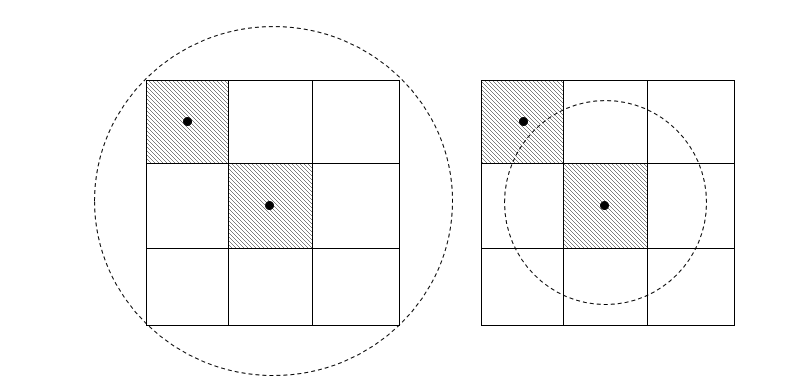
\includegraphics[width=0.35\textwidth]{figures/figure3x5}
	\caption{网格的$k$邻域的两种边界情况}\label{fig:fig35}
\end{figure}

定义10$\ Score(o, p)$:表示网格$o$在网格$p$的$k$邻域内所占的比值,满足$0 < Score(o, p) \leq 1$。

定义11$\ $局部可达密度$\left ( lrd^{'} \right )$:网格$p$的局部可达密度定义为
\begin{equation}
lrd_{k}^{'}(p) = 1 / \left ( \frac{\sum_{o\in N_k(p)}(reach-dist_k(p,o)*w_o*Score(o,p))}{\left | N_k(p) \right | } \right )
\end{equation}

定义12$\ $局部异常因子$\left ( LOF^{'} \right )$:网格$p$的局部异常因子定义为
\begin{equation}
LOF_{k}^{'}(p) = \frac{\sum_{o\in N_{k}(p)}(lrd_{k}(o)*w_o*Score(o,p)) + lrd_k(p)*w_p}{\left | N_{k}(p) \right |lrd_{k}(p)}
\end{equation}

基于以上相关定义,当数据空间被划分为足够小的网格时,映射到网格中的数据点具有相似性,将网格中的数据点用网格来代替,从而来进行异常数据检测。改进后的增量LOF快速检测算法如算法\ref{alg:mylof}所示。

\begin{algorithm}%
	\KwIn{stream data $S\  {d_1, ..., d_n}$}
	
	\KwOut{the LOF of data}
	%\SetVline
	\While{insert($d_c$)}{
		Compute $C_{d_c}$ for $d_c$\;
		Get grid $p_c$ by $C_{d_c}$\;
		\If{grid $p_c$ does not contain data}{
			$w_{p_c} = 1$\;
			Compute $kNN(p_c)$\;
			Compute $kRNN(p_c)$\;
			\For{$\forall p_j \in kNN(p_c)$}{
				Compute $reach-dist_k(p_c, p_j)$\;
			}
		}\Else{
			$w_{p_c}=w_{p_c}+1$\;
		  	Update $kNN(p_c)$\;
			\For{$\forall p_j \in kNN(p_c)$}{
				Update $reach-dist_k(p_c, p_j)$\;
			}
		}
		//Update neighbors of $p_c$ \\
		$S_{update\_k\_distance} = kRNN(p_c)$\;
		\For{$\forall p_j \in S_{update\_k\_distance}$}{
			update $k-distance(p_j)$\;
		}
		
		$S_{update\_lrd} = S_{update\_k\_distance}$\;
		\For{$\forall p_j \in S_{update\_k\_distance}$, $\forall p_i \in kNN(p_j)\setminus \left \{ p_c \right \}$}{
			$reach-dist_k(p_i, p_j) = k-distance(p_j)$\;
			\If{$p_j \in kNN(p_i)$}{
				$S_{update\_lrd} = S_{update\_lrd} \cup  \left \{ p_i \right \}$\;
			} 
		}
		$S_{update\_LOF} = S_{update\_lrd}$\;
		\For{$\forall p_m \in S_{update\_lrd}$}{
			update $lrd(p_m)$\;
			$S_{update\_LOF} = S_{update\_LOF} \cup  kRNN\left \{ p_m \right \}$\;
		}
		\For{$\forall p_l \in S_{update\_LOF}$}{
			update $LOF(p_l)$\;
		}
		compute $lrd(p_c)$\;
		compute $LOF(p_c)$\;
		$LOF(d_c) = LOF(p_c)$\;
	}
	\caption{改进的增量LOF快速检测算法}
	\label{alg:mylof}
\end{algorithm}

改进后的增量LOF快速检测算法可以解决以下问题:

(1) 流式数据的存储问题。流式数据的数据量巨大,将其存储将消耗昂贵的存储资源。而将数据空间划分为网格结构后,网格的数量是确定的,对每个网格存储其特征向量,则无论有多少流式数据,存储的空间不变,在流式数据源源不断到来后,将数据点存储在网格结构中,总的存储量不会增加,可以解决流式数据数据量大,无法存储的问题。

(2) 流式数据的异常数据检测的计算时间问题。将流式数据的数据点映射到网格中时,计算量会大大减少。因为当新来数据点时,需要计算该数据点的$k$邻域,在原本的算法中,需要计算新来数据点与已有所有数据点的距离,并将所得距离排序,找到离新来数据点最近的$k$个点,而本文的算法中,分为两种情况,一种是新来的数据点映射到的网格中之前没有数据点,此时,根据网格的空间的相邻网格的特性,计算其$k$邻域,另一种是新来的数据点所映射到的网格已经存在数据点,此时,不需要重新计算$k$邻域,只需要更新网格的特征向量,包括其$k$邻域。当数据点几百几千个时,两者计算时间差别不大,但是当数据量远远超过网格的数量时,如数据达到上万百万以及更多时,本文的算法的计算量大大减少,计算速度很大幅度地提高,计算时间快速减少。其次,在存储方式上,网格根据其坐标向量可以使用数组结构存储,数据读取迅速,也可以减少计算时间。因此,本算法可以实现流式数据的快速异常数据检测。

\section{算法加速分析}
本算法是一种快速检测算法,主要从两方面可以减少计算时间。

(1) 算法计算量方面的差异。从上文分析可知,本算法与增量的LOF算法相比,主要变化在于计算的数据量的改变。在大数据时代,数据量呈爆炸式增长,据工信部统计显示,2016年我国移动互联网接入流量达$936$万TB,同比增长$123.7\%$,市场调研机构IDC预计,未来全球数据总量年增长率将维持在$50\%$左右,到$2020$年,全球数据总量将达到$40$ZB。由此可见,数据量是巨大的。在应用场景中,流式数据到来后,数据量越来越多,计算也越来越复杂,所以,计算量和存储量是一直随着时间增长的,而在本算法中,用空间中的网格来代替数据点,数据点的多少影响的只是网格的权重,当数据到来时,有数据的网格越来越多,当全部网格都有数据后,随着时间的增长,数据量变多,但是网格的数量不会增多,所以存储量和计算量也不会再加大。

(2) 计算过程中的差异。增量的LOF算法中,每来一个数据点,都是一个全新的数据点,相关的计算都要进行,其中包括计算其$knn$和$krnn$。现有的计算数据点的$knn$的最有效的算法\upcite{Roussopoulos1995Nearest}与计算$krnn$的最有效的算法\upcite{Achtert2006Efficient}的时间复杂度都是$O( \log n)$。而本算法中,如果该网格之前已经有了数据点,则与原方法的需要计算$knn$与$krnn$相比,本算法只需要更新$knn$即可,而且更新的时间复杂度为$O(1)$。异常数据点是较少的,而大部分数据点都会聚集,当数据密集分布时,流向同一网格的数据会较多,从而减少一定量的计算量。其次,本算法的主要目的是为了检测新来的数据点是否为异常数据点,当程序运行一定时间后,数据流趋于稳定时,如果新来的数据映射到的网格权值较大,异常数据值较小,那么表明该网格内的数据点很多,那么新来的数据点基本可以确定其不是异常数据点,从而不进行各种计算,只更新该网格的权值。但是,为了防止数据流发生变化,原先不是异常的网格一段时间后因为周围网格数据点的大幅度增多而变为异常网格,每隔一段时间后,可以更新一下每个网格的特征向量。
如图\ref{fig:fig37}所示,是用大小为$100$的小数据集做的小对比实验,从中可以看出,本算法的内存使用量峰值大约为$520$MB,而增量的LOF算法的内存使用量峰值大约为$1.0$GB,而且可以看出,本算法的平均内存使用量更少,而运行时间也更短。

\begin{figure}[htbp]
	\centering                                      %居中
	\subfigure[改进的增量LOF的快速检测算法]{              %第一张子图
		\begin{minipage}{6cm}
			\label{fig:fig371}
			\centering                              %子图居中
			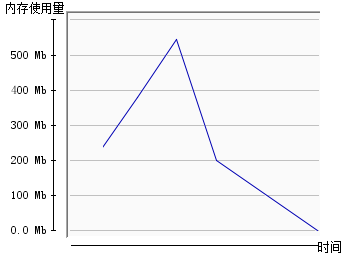
\includegraphics[width=0.7\textwidth]{figures/figure3x71}   %以pic.jpg的0.5倍大小输出
		\end{minipage}
	}
	\subfigure[增量LOF检测算法]{                  %第二张子图
		\begin{minipage}{8cm}
			\label{fig:fig372}
			\centering                                  %子图居中
			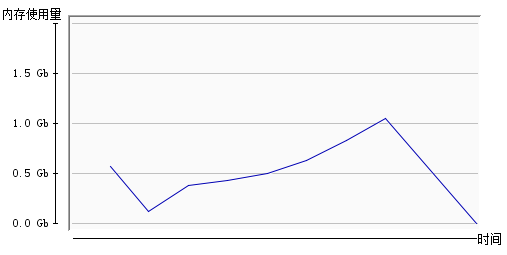
\includegraphics[width=0.8\textwidth]{figures/figure3x72}       %以pic.jpg的0.5倍大小输出
		\end{minipage}
	}\caption{内存使用量变化图(横坐标为运行时间,纵坐标为内存容量)} %                     %大图名称
	\label{fig:fig37}                                       %图片引用标记
\end{figure}

\section{本章小结}
由上可知,LOF算法可以检测数据点的局部异常因子,根据局部异常因子来判断此数据点是否是异常数据点。在流式环境下,可以使用增量的LOF算法,只计算更新新来数据点及其影响到的数据点,计算这些数据点的局部异常因子。但是流式数据数据量巨大,数据维度高,该方法无法解决大规模数据的计算与存储问题。本文提出一种新算法,将增量的LOF算法与网格相结合,并设计了网格的特征向量,以网格代替其中的数据点来进行计算。该算法不但可以减少存储空间,也可以减少计算量,实现流式数据的快速异常数据检测。为了验证本算法的可实施性和精确性以及加速效果,将在第五章进行实验验证。
